\section{曲面的基本群}
\label{ch12-sec74}

本节我们主要说明如何构造紧致连通曲面并计算它们的基本群. 我们所构造的这些曲面中, 每一个都是将某一个平面多边形区域的边界"黏合起来"而得到的商空间.

为了使这个黏合过程有章可循, 我们必须认真对待某些问题. 首先我们将对"平面多边形区域"给出一个确切的定义. 给定平面 $\mathbb{R}^{2}$ 上的一个点 $c$ 以及一个正数 $a>0$, 考虑 $\mathbb{R}^{2}$ 中以 $c$ 为圆心、以 $a$ 为半径的圆周. 给定实数的一个有限序列 $\theta_{0}<\theta_{1}<\cdots<\theta_{n}$, 其中 $n\geqslant 3$, $\theta_{n}=\theta_{0}+2\pi$, 考虑圆周上的点 $p_{i}=c+a(\cos\theta_{i},\ \sin\theta_{i})$. 这些点在圆周上按逆时针方向依次排列并且 $p_{n}=p_{0}$. 连接 $p_{i-1}$ 和 $p_{i}$ 的直线将整个平面分割成两个闭的半平面. 用 $H_{i}$ 表示其中含有所有 $p_{k}$ 的那个半平面, 则空间
\[
P=H_{1}\cap\cdots\cap H_{n}
\]
称为由这些点 $p_{i}$ 所决定的\textbf{多边形区域}(polygonal region). 这些点 $p_{i}$ 称为 $P$ 的\textbf{顶点}(vertex), 连接 $p_{i-1}$ 和 $p_{i}$ 的线段称为 $P$ 的一条\textbf{边}(edge), 以 $\operatorname{Bd}P$ 表示所有各边的并, $\operatorname{Int}P$ 表示集合 $P-\operatorname{Bd}P$. 易见, 如果 $p$ 为 $\operatorname{Int}P$ 的一个点, 则 $P$ 可以表示成所有连接点 $p$ 和 $\operatorname{Bd}P$ 中点的线段的并, 并且两条线段仅在 $p$ 点处相交.

给定 $\mathbb{R}^{2}$ 中的一条线段 $L$, $L$ 的一个\textbf{定向}(orientation)是其端点的一个排列, 倘若 $L$ 的第一个端点为 $a$, 第二个端点为 $b$, 则称 $a$ 为有向线段 $L$ 的\textbf{起点}(initial point), $b$ 为有向线段 $L$ 的\textbf{终点}(final point). 这时, 我们常称 $L$ 为一条从 $a$ 到 $b$ 的有向线段, 并且用 $L$ 上由 $a$ 指向 $b$ 的一个箭头标明 $L$ 的定向. 如果 $L'$ 是另一条由 $c$ 到 $d$ 的有向线段, 那么 $L$ 到 $L'$ 的\textbf{正线性映射}(positive linear map)是指一个同胚 $h$, 它将 $L$ 中的点 $x=(1-s)a+sb$ 映为 $L'$ 中的点 $h(x)=(1-s)c+sd$.

如果多边形区域 $P$ 的顶点 $p_{0},\ \cdots,\ p_{n}$ ($p_{0}=p_{n}$) 的个数与多边形区域 $Q$ 的顶点 $q_{0},\ \cdots,\ q_{n}$ ($q_{0}=q_{n}$) 的个数相同, 那么明显地存在一个从 $\operatorname{Bd}P$ 到 $\operatorname{Bd}Q$ 的同胚 $h$, 它将从 $p_{i-1}$ 到 $p_{i}$ 的边按正线性的方式映射到从 $q_{i-1}$ 到 $q_{i}$ 的边上. 如果 $p$ 和 $q$ 分别为 $\operatorname{Int}P$ 和 $\operatorname{Int}Q$ 中的取定的点, 那么上述同胚可以扩充为一个从 $P$ 到 $Q$ 的同胚, 它将连接 $p$ 和 $\operatorname{Bd}P$ 中一点 $x$ 的线段线性地映到连接 $q$ 和 $h(x)$ 的线段上. 参见\cref{ch12-fig-74-1}.

\begin{definition}[标记与黏合]
\label{definition:ch12-labelling-pasting}
设 $P$ 是一个平面多边形区域. $P$ 的诸边的一个\textbf{标记}(labelling)是指从 $P$ 的边构成的集合到某一个集合 $S$ 的映射, 集合 $S$ 叫做\textbf{标签}(label)集. 对 $P$ 的每一条边给定了一个定向, 又给定了 $P$ 的诸边的一个标记, 我们在 $P$ 中定义一个等价关系如下: $\operatorname{Int}P$ 中的每一个点仅与其自身等价. 对于具有相同标签的 $P$ 的两条边, 设 $h$ 是从其中某一条边到另一条边上的正线性映射, 则定义前一条边上的点 $x$ 与另一边上的点 $h(x)$ 等价. 这样定义的关系的确是 $P$ 中的一个等价关系. 通过这个等价关系而得到的商空间 $X$ 叫做按照给定的定向和给定的标记\textbf{黏合 $P$ 的各边}(pasting the edges of $P$)得到的商空间.
\end{definition}

\par
\begin{figure}[htbp]
\centering
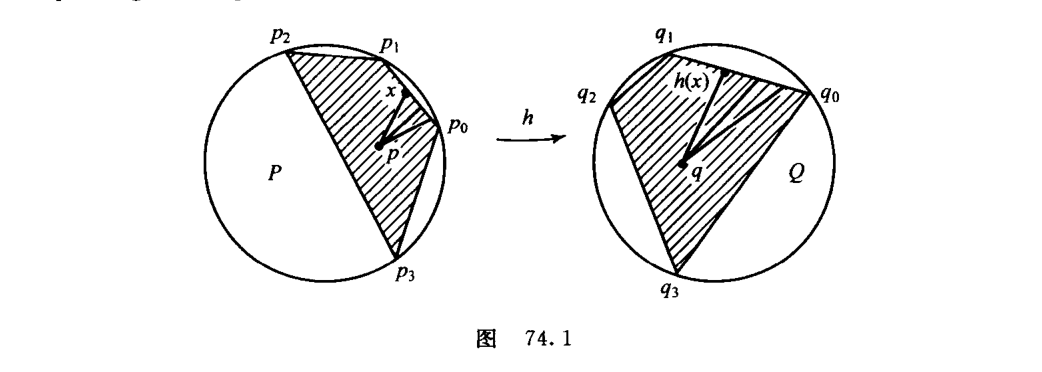
\includegraphics[width=0.7\textwidth]{image/fig-74-1.png}
\caption{多边形区域之间的同胚扩充.}
\label{ch12-fig-74-1}
\end{figure}

\begin{example}[三角形黏合成球面]
\label{example:ch12-triangle-sphere}
考虑由\cref{ch12-fig-74-2} 给出的三角形区域的各边的定向和标记. 这个图说明我们可以得到一个与单位球同胚的商空间.
\end{example}

\par
\begin{figure}[htbp]
\centering
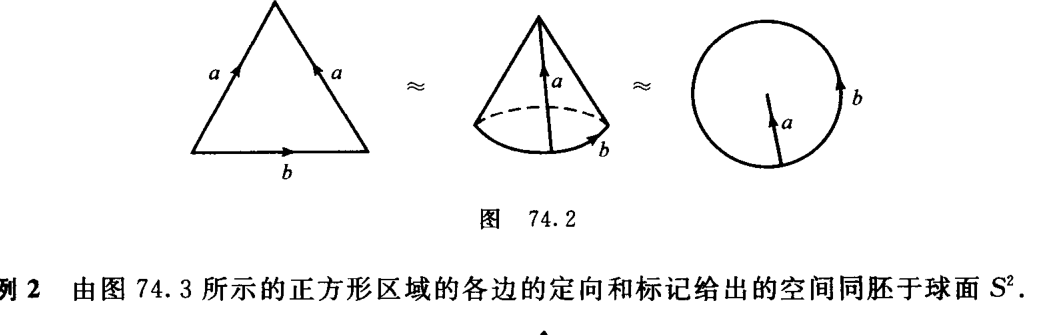
\includegraphics[width=0.7\textwidth]{image/fig-74-2.png}
\caption{三角形区域黏合为与单位球同胚的空间.}
\label{ch12-fig-74-2}
\end{figure}

\begin{example}[正方形黏合成球面]
\label{example:ch12-square-sphere}
由\cref{ch12-fig-74-3} 所示的正方形区域的各边的定向和标记给出的空间同胚于球面 $S^{2}$.
\end{example}

\par
\begin{figure}[htbp]
\centering
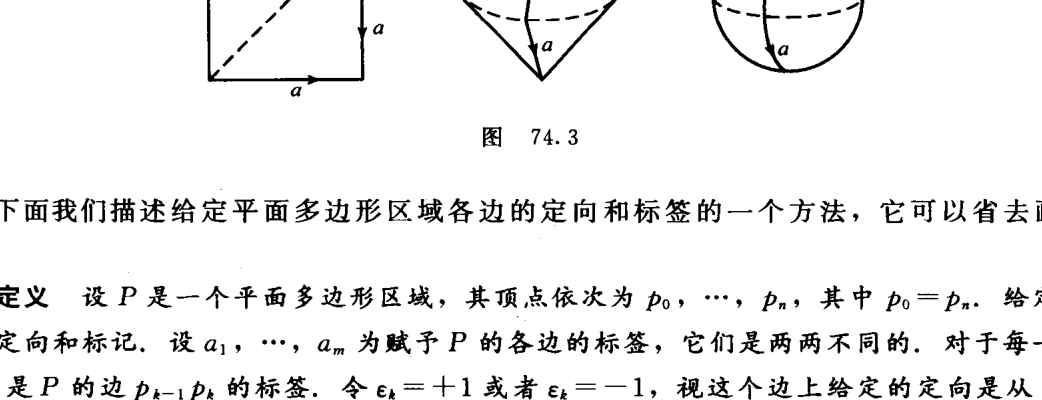
\includegraphics[width=0.7\textwidth]{image/fig-74-3.png}
\caption{正方形区域黏合为球面 $S^{2}$.}
\label{ch12-fig-74-3}
\end{figure}

下面我们描述给定平面多边形区域各边的定向和标签的一个方法, 它可以省去画图的麻烦.

\begin{definition}[标记表]
\label{definition:ch12-labelling-scheme}
设 $P$ 是一个平面多边形区域, 其顶点依次为 $p_{0},\ \cdots,\ p_{n}$, 其中 $p_{0}=p_{n}$. 给定 $P$ 各边的定向和标记. 设 $a_{1},\ \cdots,\ a_{m}$ 为赋予 $P$ 的各边的标签, 它们是两两不同的. 对于每一个 $k$, 设 $a_{i_{k}}$ 是 $P$ 的边 $p_{k-1}p_{k}$ 的标签. 令 $\varepsilon_{k}=+1$ 或者 $\varepsilon_{k}=-1$, 视这个边上给定的定向是从 $p_{k-1}$ 到 $p_{k}$ 还是相反而定. 这时, $P$ 的边的条数、各边的定向和标记完全由以下符号定义:
\[
w=(a_{i_{1}})^{\varepsilon_{1}}(a_{i_{2}})^{\varepsilon_{2}}\cdots(a_{i_{n}})^{\varepsilon_{n}}.
\]
我们称形式符号 $w$ 为 $P$ 的诸边的一个\textbf{长度为 $n$ 的标记表}(labelling scheme of length $n$), 它只是由一系列标签和指数 $+1$ 或 $-1$ 组成.
\end{definition}

当我们给定一个标记表的时候, 通常省略等于 $+1$ 的指数. 例如, 在\cref{example:ch12-triangle-sphere} 中, 如果取 $p_{0}$ 为三角形最高顶点的话, 则给出的各边的定向和标记便可以用标记表 $a^{-1}ba$ 来刻画. 如果我们选择其他顶点为 $p_{0}$, 则得到标记表 $baa^{-1}$ 或者 $aa^{-1}b$.

类似地, 对于\cref{example:ch12-square-sphere} 中所示的定向和标记可以用 $aa^{-1}bb^{-1}$ 来刻画 (如果从正方形左下角的顶点开始).

显然, 对于标记表各项的一个轮换, 不至于使得由这个标记表所决定的空间 $X$ 在同胚的意义下有所改变. 稍后, 我们还将考虑对标记表作其他修改, 要求这种修改使空间 $X$ 在同胚的意义下不变.

\begin{example}[环面]
\label{example:ch12-torus}
此前, 我们曾经讨论过环面可以作为一个商空间通过商映射 $p\times p\colon I\times I\to S^{1}\times S^{1}$ 来得到. 它也可以通过\cref{ch12-fig-74-4} 所示的正方形各边的定向和标记获得. 其标记表可取为 $aba^{-1}b^{-1}$.
\end{example}

\par
\begin{figure}[htbp]
\centering
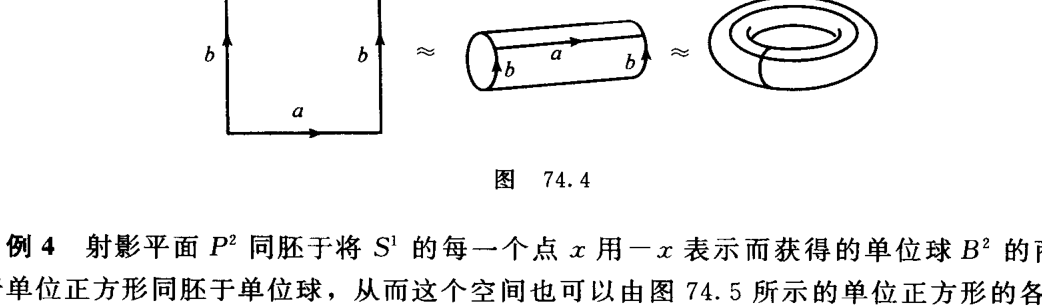
\includegraphics[width=0.65\textwidth]{image/fig-74-4.png}
\caption{环面的标记表 $aba^{-1}b^{-1}$.}
\label{ch12-fig-74-4}
\end{figure}

\begin{example}[射影平面]
\label{example:ch12-projective-plane}
射影平面 $P^{2}$ 同胚于将 $S^{1}$ 的每一个点 $x$ 用 $-x$ 表示而获得的单位球 $B^{2}$ 的商空间. 由于单位正方形同胚于单位球, 从而这个空间也可以由\cref{ch12-fig-74-5} 所示的单位正方形的各边的定向和标记来表示. 其标记表可取为 $abab$.
\end{example}

\par
\begin{figure}[htbp]
\centering
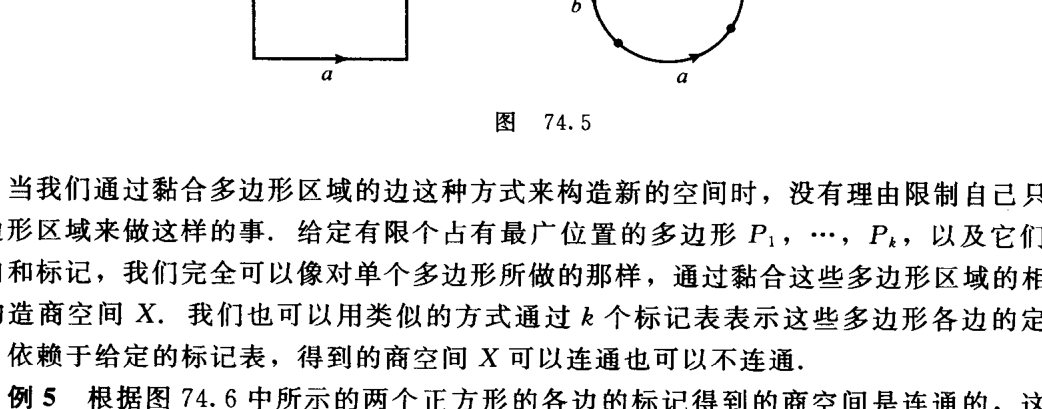
\includegraphics[width=0.75\textwidth]{image/fig-74-5.png}
\caption{射影平面 $P^{2}$ 的标记表 $abab$.}
\label{ch12-fig-74-5}
\end{figure}

当我们通过黏合多边形区域的边这种方式来构造新的空间时, 没有理由限制自己只对单个多边形区域来做这样的事. 给定有限个占有最广位置的多边形 $P_{1},\ \cdots,\ P_{k}$, 以及它们各边的定向和标记, 我们完全可以像对单个多边形所做的那样, 通过黏合这些多边形区域的相应的边来构造商空间 $X$. 我们也可以用类似的方式通过 $k$ 个标记表表示这些多边形各边的定向和标记. 依赖于给定的标记表, 得到的商空间 $X$ 可以连通也可以不连通.

\begin{example}[Möbius 带]
\label{example:ch12-mobius}
根据\cref{ch12-fig-74-6} 中所示的两个正方形的各边的标记得到的商空间是连通的, 这个空间称为 \textbf{Möbius 带}(Möbius band). 可以验证, 这个空间也可以通过一个带有标记表 $abac$ 的正方形来构造.
\end{example}

\par
\begin{figure}[htbp]
\centering
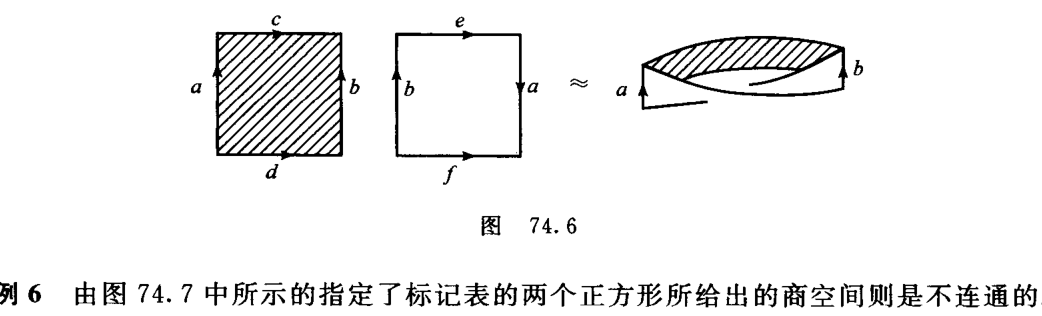
\includegraphics[width=0.8\textwidth]{image/fig-74-6.png}
\caption{Möbius 带.}
\label{ch12-fig-74-6}
\end{figure}

\begin{example}[不连通的商空间]
\label{example:ch12-disconnected}
由\cref{ch12-fig-74-7} 中所示的指定了标记表的两个正方形所给出的商空间则是不连通的.
\end{example}

\par
\begin{figure}[htbp]
\centering
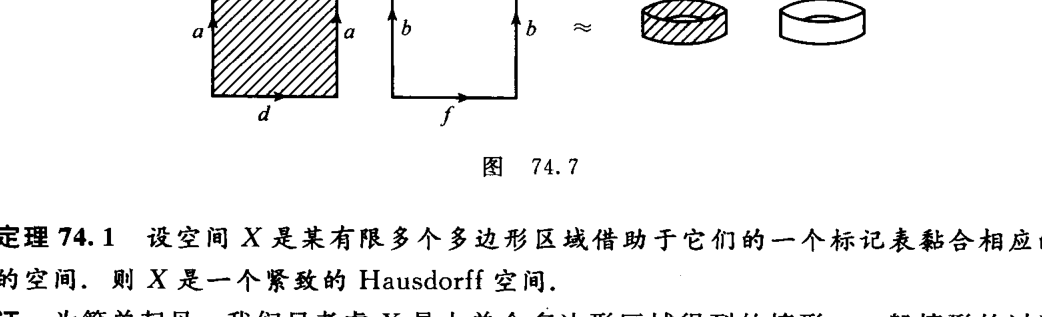
\includegraphics[width=0.8\textwidth]{image/fig-74-7.png}
\caption{两个互不连通的商空间.}
\label{ch12-fig-74-7}
\end{figure}

\begin{theorem}[黏合边所得空间是紧致 Hausdorff 空间]
\label{theorem:ch12-compact-hausdorff}
设空间 $X$ 是某有限多个多边形区域借助于它们的一个标记表黏合相应的边所得到的空间. 则 $X$ 是一个紧致的 Hausdorff 空间.
\end{theorem}

\begin{proof}
为简单起见, 我们只考虑 $X$ 是由单个多边形区域得到的情形. 一般情形的讨论与此相仿.

由于商映射是连续的, 显然 $X$ 是紧致的. 为了证明 $X$ 是一个 Hausdorff 空间, 只需要证明商映射 $\pi$ 是闭映射 (参见引理 73.3). 为此, 我们需验证对于 $P$ 的每一个闭集 $C$, $\pi^{-1}\pi(C)$ 为 $P$ 中的闭集. 集合 $\pi^{-1}\pi(C)$ 由 $C$ 的点以及 $P$ 中经 $\pi$ 黏合到 $C$ 中的那些点组成. 这些点容易确定. 对于 $P$ 的一条边 $e$, 用 $C_{e}$ 表示 $P$ 的紧致子空间 $C\cap e$. 如果 $e_{i}$ 是 $P$ 中被黏合到 $e$ 的边, $h_{i}\colon e_{i}\to e$ 为黏合同胚, 则集合 $D_{e}=\pi^{-1}\pi(C)\cap e$ 包含着空间 $h_{i}(C_{e_{i}})$. 事实上, $D_{e}$ 等于 $C_{e}$ 与所有 $h_{i}(C_{e_{i}})$ 的并, 其中 $e_{i}$ 取遍所有 $P$ 被黏合到 $e$ 的边. 这个并是紧致的, 因此它是 $e$ 中的闭集, 也是 $P$ 中的闭集.

由于 $\pi^{-1}\pi(C)$ 是集合 $C$ 和诸集合 $D_{e}$ 的并, 其中 $e$ 取遍 $P$ 的所有边, 因此它是 $P$ 中的闭集. 这便是我们需要证明的.
\end{proof}

注意, 如果 $X$ 是由多边形区域通过边的黏合而得到的空间, 那么商映射 $\pi$ 可能会将多边形的所有顶点映射为 $X$ 上的某一个点, 也可能不是这样. 对\cref{example:ch12-torus} 中的环面, 其商映射便满足这个条件, 而\cref{example:ch12-triangle-sphere} 和\cref{example:ch12-square-sphere} 中球和曲面相应的商映射却不满足这个条件. 遇到满足这个条件的商映射 $\pi$, 我们将感到十分欣慰, 因为这时 $X$ 的基本群容易计算.

\begin{theorem}[黏合空间的基本群]
\label{theorem:ch12-pasted-space-pi1}
设 $P$ 是一个多边形区域,
\[
w=(a_{i_{1}})^{\varepsilon_{1}}\cdots(a_{i_{n}})^{\varepsilon_{n}}
\]
为 $P$ 的各边的一个标记表, $X$ 是相应的商空间, $\pi\colon P\to X$ 是相应的商映射. 如果 $\pi$ 将 $P$ 的所有顶点映射到 $X$ 的一个点 $x_{0}$, 并且 $a_{1},\ \cdots,\ a_{k}$ 为标记表中所有互不相同的标签, 则 $\pi_{1}(X,\ x_{0})$ 同构于具有 $k$ 个生成元 $\alpha_{1},\ \cdots,\ \alpha_{k}$ 的自由群关于包含着元素
\[
(\alpha_{i_{1}})^{\varepsilon_{1}}\cdots(\alpha_{i_{n}})^{\varepsilon_{n}}
\]
的最小正规子群的商群.
\end{theorem}

\begin{proof}
这里给出的证明与第 73 节中对于环面给出的证明相仿. 因为 $\pi$ 将 $P$ 的所有顶点映射为 $X$ 的一个点, 从而空间 $A=\pi(\operatorname{Bd}P)$ 是 $k$ 个圆周的束. 对于每一个 $i$ 选取标签为 $a_{i}$ 的 $P$ 的一条边, 规定其上的定向为逆时针方向. 设 $f_{i}$ 为从 $I$ 到这条边的正线性映射, 并且令 $g_{i}=\pi\circ f_{i}$, 则回路 $g_{1},\ \cdots,\ g_{k}$ 代表 $\pi_{1}(A,\ x_{0})$ 的自由生成元. 绕着 $\operatorname{Bd}P$ 按逆时针方向转了一圈的回路 $f$ 生成 $\operatorname{Bd}P$ 的基本群. 回路 $\pi\circ f$ 等于回路
\[
(g_{i_{1}})^{\varepsilon_{1}}*\cdots*(g_{i_{n}})^{\varepsilon_{n}}.
\]
根据定理 72.1, 该定理成立.
\end{proof}

\begin{definition}[ $n$-重环面]
\label{definition:ch12-n-fold-torus}
考虑由 $4n$-边形区域借助于标记表
\[
(a_{1}b_{1}a_{1}^{-1}b_{1}^{-1})(a_{2}b_{2}a_{2}^{-1}b_{2}^{-1})\cdots(a_{n}b_{n}a_{n}^{-1}b_{n}^{-1})
\]
所得到的空间. 此空间称为\textbf{环面的 $n$-重连通和}($n$-fold connected sum of tori), 或者简称为\textbf{$n$-重环面}($n$-fold torus), 记作 $T\#\cdots\#T$.
\end{definition}

$2$-重环面如\cref{ch12-fig-74-8} 所示. 如果将多边形区域 $P$ 沿图示的直线 $c$ 割开, 则分成两块中的每一块都是一个挖掉了一个开圆盘的环面. 若再将这样两个曲面沿曲线 $c$ 黏合起来, 则又得到了第 60 节中给出的空间, 这里称为\textbf{双重环面}(double torus). 相仿的讨论说明 $3$-重环面可以画成\cref{ch12-fig-74-9} 所示的曲面.

\par
\begin{figure}[htbp]
\centering
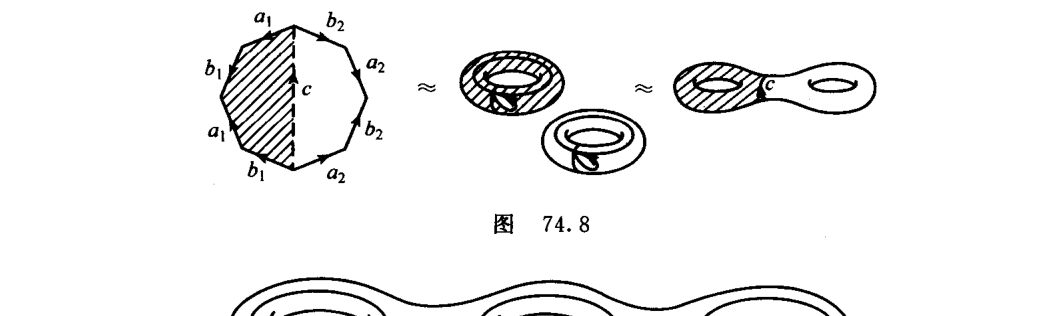
\includegraphics[width=0.85\textwidth]{image/fig-74-8.png}
\caption{双重环面.}
\label{ch12-fig-74-8}
\end{figure}

\par
\begin{figure}[htbp]
\centering
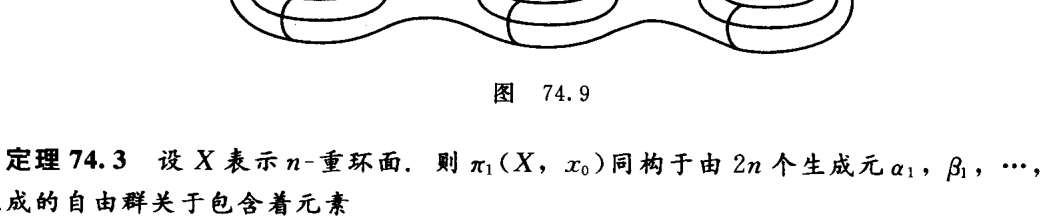
\includegraphics[width=0.85\textwidth]{image/fig-74-9.png}
\caption{$3$-重环面.}
\label{ch12-fig-74-9}
\end{figure}

\begin{theorem}[ $n$-重环面的基本群]
\label{theorem:ch12-n-fold-torus-pi1}
设 $X$ 表示 $n$-重环面. 则 $\pi_{1}(X,\ x_{0})$ 同构于由 $2n$ 个生成元 $\alpha_{1},\ \beta_{1},\ \cdots,\ \alpha_{n},\ \beta_{n}$ 所生成的自由群关于包含着元素
\[
[\alpha_{1},\beta_{1}][\alpha_{2},\beta_{2}]\cdots[\alpha_{n},\beta_{n}]
\]
的最小正规子群的商群, 其中 $[\alpha,\ \beta]=\alpha\beta\alpha^{-1}\beta^{-1}$.
\end{theorem}

\begin{proof}
为应用 \cref{theorem:ch12-pasted-space-pi1}, 必须证明对于 $X$ 的给定的标记表, 多边形区域的所有顶点都属于同一等价类. 我们将证明留给读者.
\end{proof}

\begin{definition}[ $m$-重射影平面]
\label{definition:ch12-m-fold-projective}
设 $m>1$. 考虑由平面上的 $2m$-边多边形区域 $P$ 借助于标记表
\[
(a_{1}a_{1})(a_{2}a_{2})\cdots(a_{m}a_{m})
\]
所得到的空间. 此空间称为\textbf{射影平面的 $m$-重连通和}($m$-fold connected sum of projective plane), 或简称为\textbf{$m$-重射影平面}($m$-fold projective plane), 记作 $P^{2}\#\cdots\#P^{2}$.
\end{definition}

$2$-重射影平面 $P^{2}\#P^{2}$ 画在\cref{ch12-fig-74-10} 中. 此图说明如何从两个射影平面构造这个空间. 我们先从每一个射影平面上挖掉一个开圆盘, 然后沿所挖掉圆盘的边界将两个空间黏合. 与 $P^{2}$ 的情形类似, 我们无法在 $\mathbb{R}^{3}$ 中画出 $m$-重射影平面, 事实上, 它不能嵌入到 $\mathbb{R}^{3}$ 中. 然而, 有时我们也把它画成 $\mathbb{R}^{3}$ 中自交的曲面. (称之为浸入曲面, 以区别于嵌入曲面.)在习题中对此进行探讨.

\par
\begin{figure}[htbp]
\centering
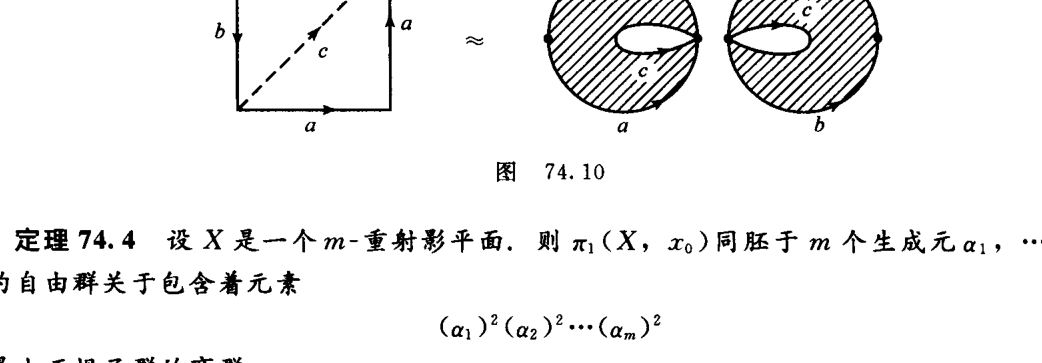
\includegraphics[width=0.85\textwidth]{image/fig-74-10.png}
\caption{$P^{2}\#P^{2}$ 的构造.}
\label{ch12-fig-74-10}
\end{figure}

\begin{theorem}[ $m$-重射影平面的基本群]
\label{theorem:ch12-m-fold-projective-pi1}
设 $X$ 是一个 $m$-重射影平面. 则 $\pi_{1}(X,\ x_{0})$ 同胚于 $m$ 个生成元 $\alpha_{1},\ \cdots,\ \alpha_{m}$ 生成的自由群关于包含着元素
\[
(\alpha_{1})^{2}(\alpha_{2})^{2}\cdots(\alpha_{m})^{2}
\]
的最小正规子群的商群.
\end{theorem}

\begin{proof}
只需验证对于 $X$ 的给定的标记表, 多边形区域的所有顶点都属于同一等价类. 我们将证明留给读者.
\end{proof}

有许多办法构造紧致曲面. 比如, 可以在 $P^{2}$ 和 $T$ 上各自挖掉一个开圆盘, 而后再将它们沿所挖掉的圆盘的边界黏合起来. 可以验证上述空间可由 $6$-边形并借助于标记表 $aabcb^{-1}c^{-1}$ 得到. 然而, 我们将不再讨论它, 因为我们已经得到紧致连通曲面的一个完全列表. 也就是说, 我们即将给出曲面分类定理.

\begin{exercise}
\label{exercise:ch12-sec74-01}
给出 $P^{2}\#T$ 的基本群的一个表示.
\end{exercise}

\begin{exercise}
\label{exercise:ch12-sec74-02}
考虑由 $7$-边形区域借助于标记表 $abaaab^{-1}a^{-1}$ 所得到的空间 $X$. 证明 $X$ 的基本群是两个循环群的自由积. [提示: 参见定理 68.7.]
\end{exercise}

\begin{exercise}
\label{exercise:ch12-sec74-03}
\textbf{Klein 瓶}(Klein bottle) $K$ 是由矩形区域借助于标记表 $aba^{-1}b$ 所得到的空间, \cref{ch12-fig-74-11} 说明如何将 $K$ 画成一个 $\mathbb{R}^{3}$ 中的浸入曲面.
\begin{enumerate}[(a)]
\item 给出 $K$ 的基本群的一个表示.
\item 给出一个二重覆盖映射 $p\colon T\to K$, 其中 $T$ 为环面. 描述其基本群之间的诱导同态.
\end{enumerate}
\end{exercise}

\par
\begin{figure}[htbp]
\centering
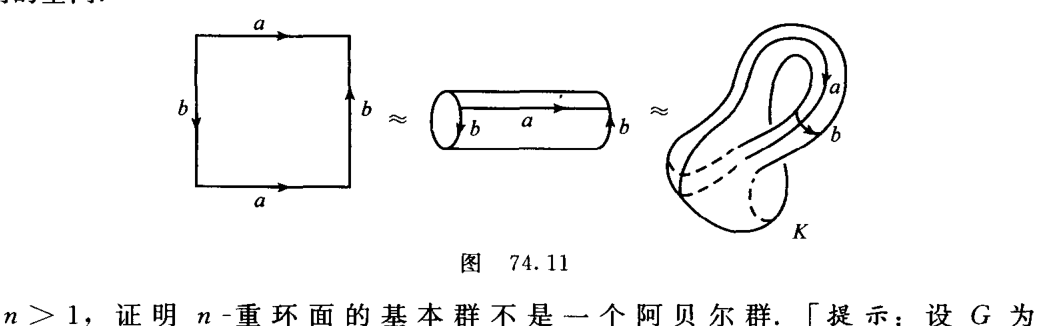
\includegraphics[width=0.7\textwidth]{image/fig-74-11.png}
\caption{Klein 瓶 $K$.}
\label{ch12-fig-74-11}
\end{figure}

\begin{exercise}
\label{exercise:ch12-sec74-04}
\begin{enumerate}[(a)]
\item 证明 Klein 瓶同胚于 $P^{2}\#P^{2}$. [提示: 在\cref{ch12-fig-74-11} 中沿对角线将矩形剪开, 将其中的一个三角形区域翻转, 然后再将两个区域中以 $b$ 为标签的边黏合起来.]
\item 说明如何将 $4$-重射影平面画成 $\mathbb{R}^{3}$ 中的浸入曲面.
\end{enumerate}
\end{exercise}

\begin{exercise}
\label{exercise:ch12-sec74-05}
Möbius 带 $M$ 叫做"有边曲面", 它不是一个曲面. 证明 $M$ 同胚于从 $P^{2}$ 中挖掉一个开圆盘而得到的空间.
\end{exercise}

\begin{exercise}
\label{exercise:ch12-sec74-06}
若 $n>1$, 证明 $n$-重环面的基本群不是一个阿贝尔群. [提示: 设 $G$ 为集合 $\{\alpha_{1},\ \beta_{1},\ \cdots,\ \alpha_{n},\ \beta_{n}\}$ 上的自由群, $F$ 为集合 $\{\gamma,\ \delta\}$ 上的自由群. 考虑从 $G$ 到 $F$ 中的同态, 它将 $\alpha_{1}$ 和 $\beta_{1}$ 映为 $\gamma$, 并且将其余的 $\alpha_{i}$ 和 $\beta_{i}$ 映为 $\delta$.]
\end{exercise}

\begin{exercise}
\label{exercise:ch12-sec74-07}
若 $m>1$, 证明 $m$-重射影平面的基本群不是一个阿贝尔群. [提示: 存在一个从这个基本群到群 $\mathbb{Z}/2*\mathbb{Z}/2$ 的同态.]
\end{exercise}
